\documentclass{article}

% Basic packages
\usepackage[utf8]{inputenc}
\usepackage[T1]{fontenc}
\usepackage{amsmath}
\usepackage{amssymb}
\usepackage{graphicx}
\usepackage{hyperref}
\usepackage{geometry}

\author{Usman Traore}
\title{Laboratory Report No. 1}

\begin{document}
\maketitle
\pagebreak

\section{Work Objective}
The objective of this laboratory work is the installation of TeX Live.

\section{Theoretical Introduction}

\subsection{Installing TeX Live}

\begin{itemize}
\item TeX Live — the most complete LaTeX distribution, supported by the TeX community.
\item Supports a large number of operating systems.
\item Developed since 1996.
\item Based on the teTeX distribution.
\item MacTeX — version for MacOS.
\item Main page: \url{https://www.tug.org/texlive/}.
\item TeX Live — distribution with continuous updates within the annual distribution version.
\end{itemize}

\subsubsection{Installation from system packages [1]}
\begin{itemize}
\item Ubuntu: \texttt{apt install texlive-full}
\item Windows: Use the Chocolatey package manager: \texttt{choco install texlive}
\end{itemize}

\subsubsection{Manual installation}
\begin{itemize}
\item Links on the website lead to mirrors. The mirror is selected automatically.
\item Download the installer:
\item Unix: \url{https://mirror.ctan.org/systems/texlive/tlnet/install-tl-unx.tar.gz}
\begin{verbatim}
cd /tmp/
wget https://mirror.ctan.org/systems/texlive/tlnet/install-tl-unx.tar.gz
\end{verbatim}
\item Windows: \url{https://mirror.ctan.org/systems/texlive/tlnet/install-tl-windows.exe}
\item For Windows: run the executable file and install.
\item For Linux:
\item Extract the downloaded file: \texttt{tar xzvf install-tl-unx.tar.gz}
\item Go to the extracted directory and run the installer:
\begin{verbatim}
cd install-tl-[0-9]*
sudo ./install-tl
\end{verbatim}
\item It is recommended to create links to executables in the \texttt{/usr/local/bin} directory. To do this, in the console version of the utility, select option O, then L. To return to the previous menu, use R.
\end{itemize}

\subsubsection{Updating to the next TeX Live version}
It is recommended to install the new TeX Live version separately.
\begin{itemize}
\item But you can perform a manual update using the existing installation.
\item Suppose our architecture is x86\_64-linux.
\item If you created symbolic links in system directories (through the installer option or \texttt{tlmgr path add}), remove them:
\begin{verbatim}
tlmgr path remove
\end{verbatim}
\item Move the entire TeX Live directory according to the new version, for example:
\begin{verbatim}
mv /usr/local/texlive/2024/ /usr/local/texlive/2025
\end{verbatim}
\item Remove package backups:
\begin{verbatim}
rm /usr/local/texlive/2025/tlpkg/backups/*
\end{verbatim}
\item Create links to executables:
\begin{verbatim}
/usr/local/texlive/2025/bin/x86_64-linux/tlmgr path add
\end{verbatim}
\item Download the latest version of the \texttt{update-tlmgr-latest.sh} script:
\begin{verbatim}
wget https://mirror.ctan.org/systems/texlive/tlnet/update-tlmgr-latest.sh \
-O /tmp/update-tlmgr-latest.sh
\end{verbatim}
\item Run the script:
\begin{verbatim}
sh /tmp/update-tlmgr-latest.sh --upgrade
\end{verbatim}
\item If you don't want to use the default repository to download new files, replace it:
\begin{verbatim}
tlmgr option repository <reponame>
\end{verbatim}
\item Update the TeX Live package manager:
\begin{verbatim}
tlmgr update --self
\end{verbatim}
\item Update TeX Live packages:
\begin{verbatim}
tlmgr update --all
\end{verbatim}
\item Install symbolic links to executables in system directories (\texttt{/usr/local/bin}):
\begin{verbatim}
tlmgr path add
\end{verbatim}
\end{itemize}

\subsection{LaTeX Basics}
\begin{itemize}
\item You can recreate the lualatex cache under the user:
\begin{verbatim}
mv ~/.texlive2024 ~/.texlive2025
luaotfload-tool -fu
\end{verbatim}
\item If you don't do this, the cache will be recreated on the first run of lualatex.
\end{itemize}

\section{Laboratory Work Execution}

\subsection{Installing and Configuring TeX Live}

Figures~\ref{fig:im1} and~\ref{fig:im2} show the TeX Live installation steps.

\subsection{Compilation Results and Files Created by TeX Live}

Figures~\ref{fig:im3} and~\ref{fig:im4} show the compilation results and created files.

\section{Conclusions}
Thus, the objective was achieved — TeX Live has been installed.

\section{Bibliography}

\begin{enumerate}
\item Zhdanov O., Ushakov Yu. Cryptographic methods of information protection. Lecture 2: Primality testing and factorization algorithms. NOU "INTUIT" \url{https://intuit.ru/studies/courses/13837/1234/lecture/31191}, 2014.
\end{enumerate}

\begin{figure}[!h]
\centering
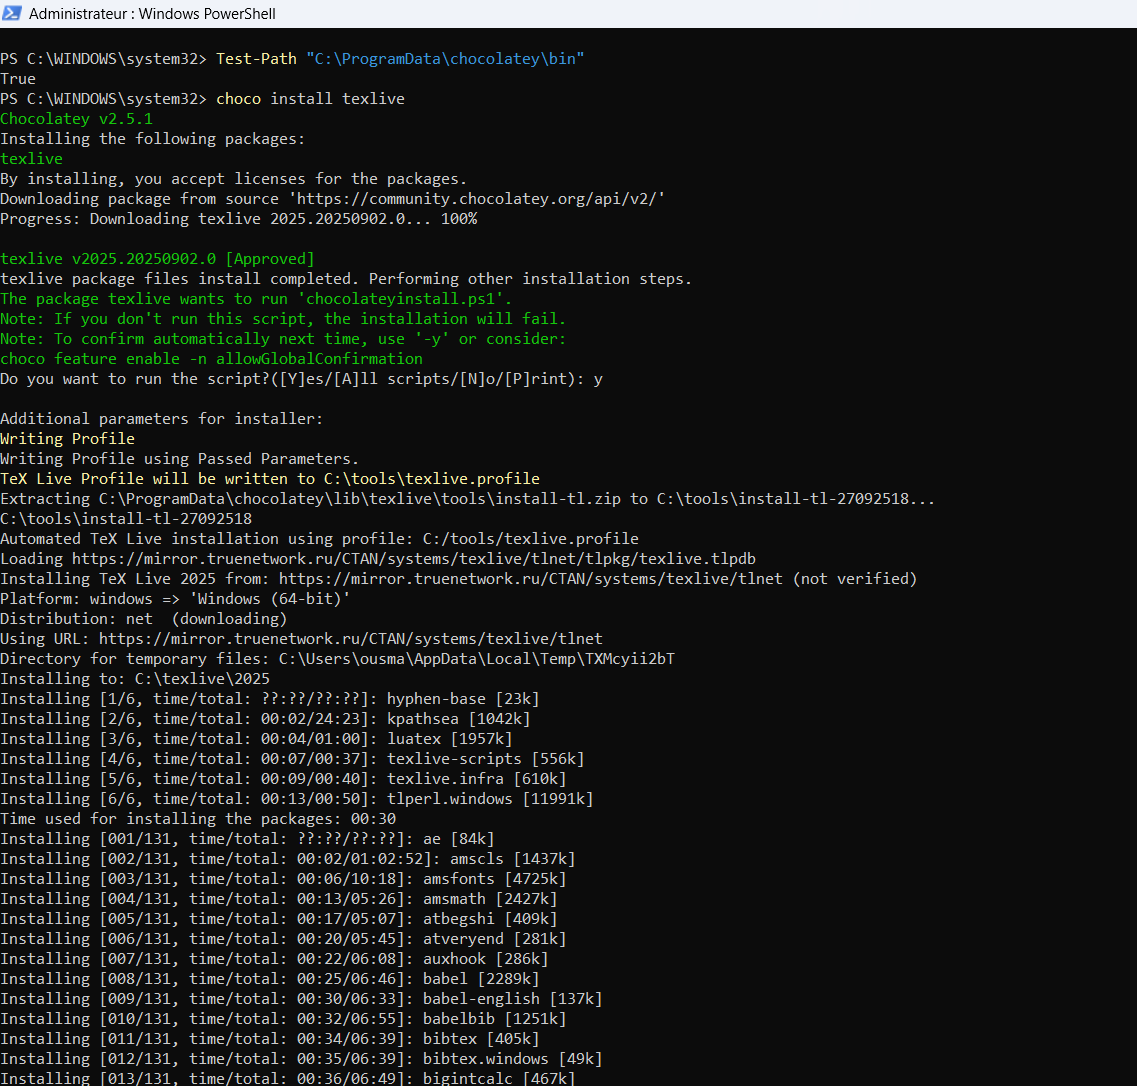
\includegraphics[width=0.8\textwidth]{im1.png}
\caption{First stage of TeX Live installation}
\label{fig:im1}
\end{figure}

\begin{figure}[!h]
\centering
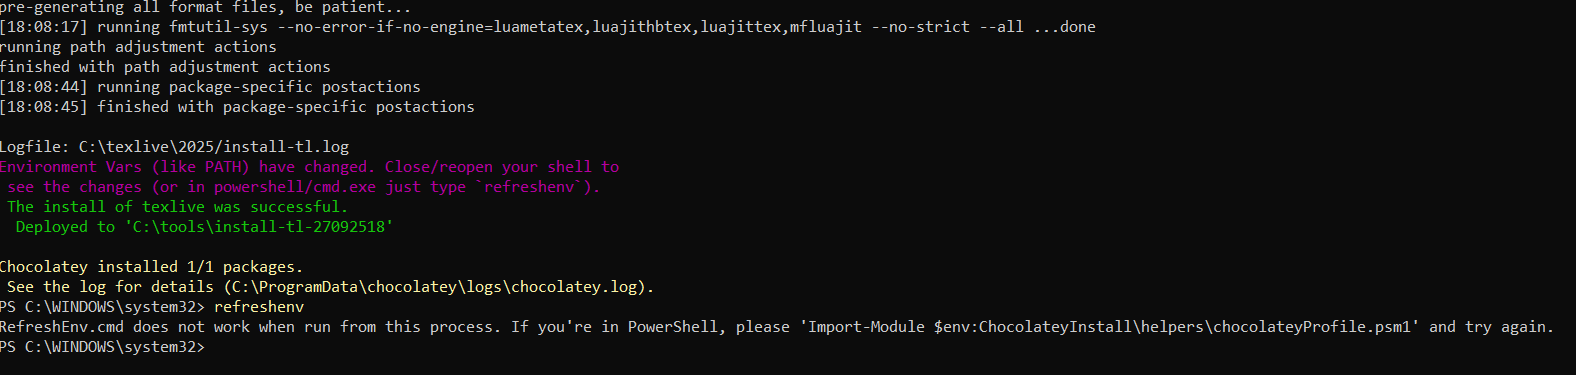
\includegraphics[width=0.8\textwidth]{im1_2.png}
\caption{Second stage of TeX Live installation}
\label{fig:im2}
\end{figure}

\begin{figure}[!h]
\centering
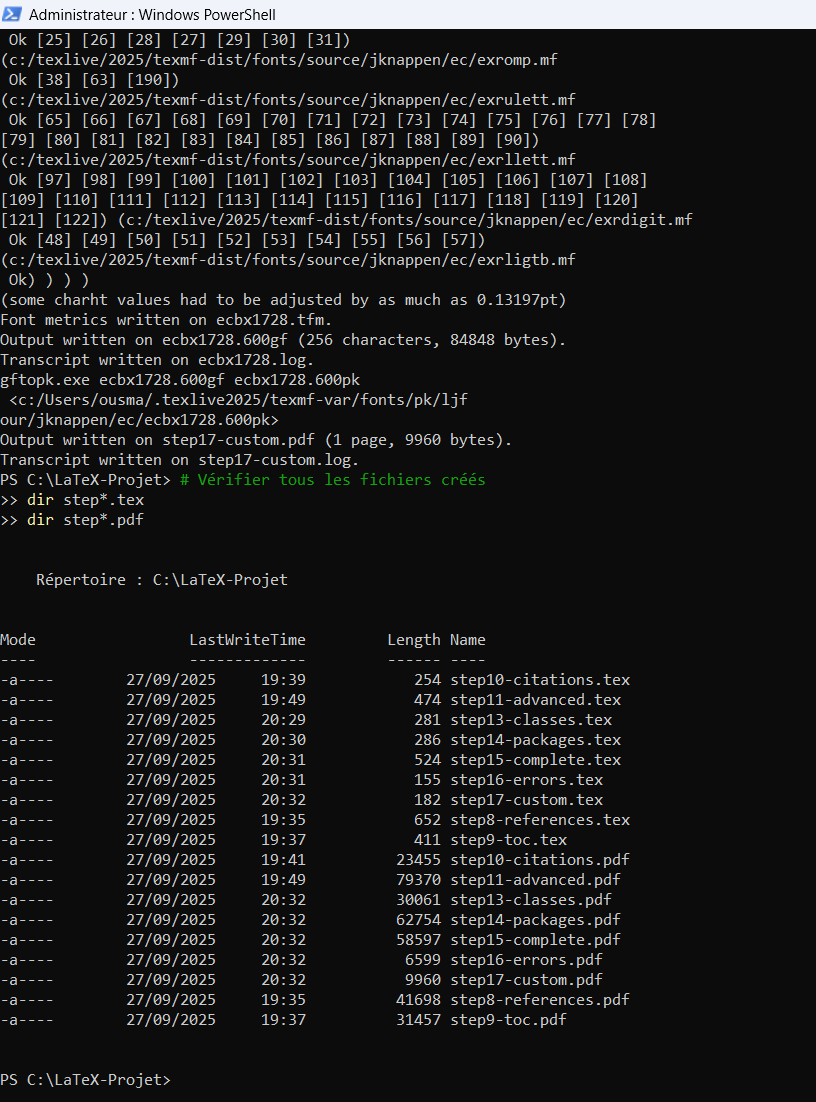
\includegraphics[width=0.8\textwidth]{im2.png}
\caption{Compilation results}
\label{fig:im3}
\end{figure}

\begin{figure}[!h]
\centering
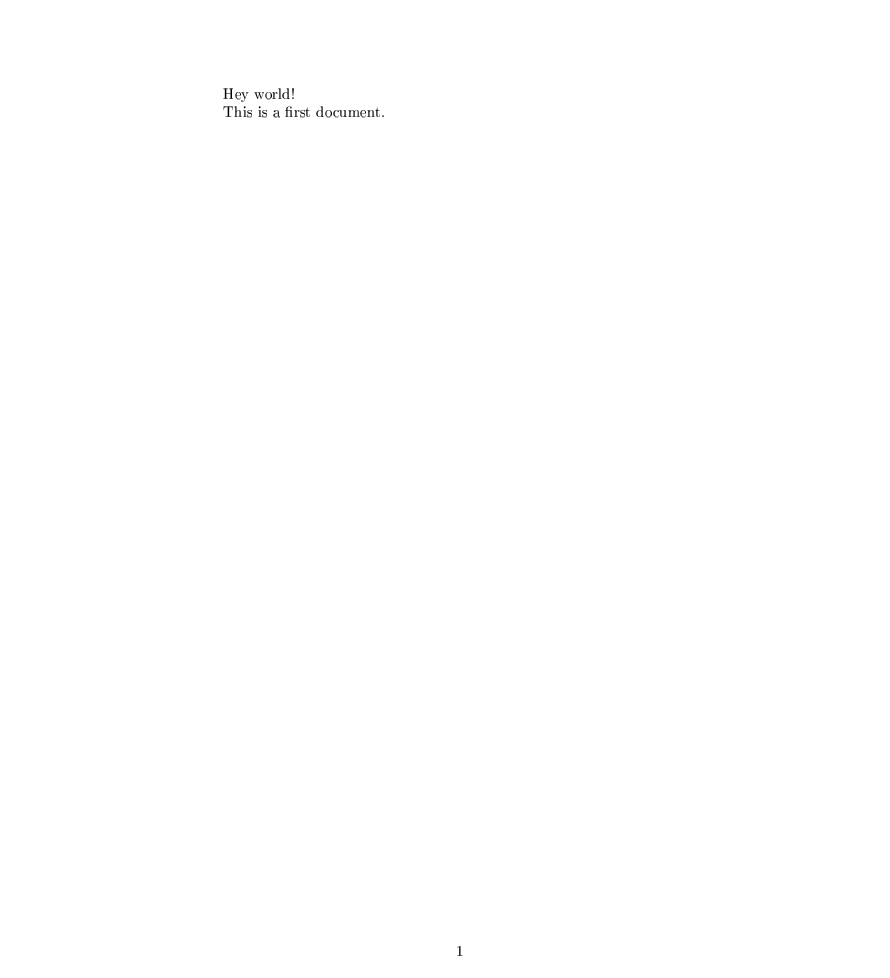
\includegraphics[width=0.8\textwidth]{im2_2.png}
\caption{Created files}
\label{fig:im4}
\end{figure}

\end{document}